The data samples used for the analyses were the FAST and CENT$\_$woSDD samples from periods LHC16q and LHC16t (AOD samples). The reason for this choice is explained later on, in this section. It was verified, by looking at D-meson and track $\eta$ and $\varphi$ distributions, and at the mixed-event correlation distributions for each subsamples, that no visible differences arose for the four periods, hence it was possible to perform the analysis directly on the merged samples without any bias.

The Monte Carlo productions adopted for this study were:
 \begin{enumerate}
 \item LHC17d2a$\_$fast$\_$new, a HIJING production with enrichment, for each event, of c or b quarks and their decay chains, performed by PYTHIA6 with Perugia2011 tune, and with forced hadronic decays of the charmed hadrons. This production was used for D-meson efficiency evaluation, purity estimation and Monte Carlo closure test.
 \item LHC17a2b$\_$cent$\_$woSDD and LHC17a2b$\_$fast, minimum-bias samples produced with DPMJET generator, used for the evaluation of the tracking efficiencies.
\end{enumerate}

Table 1 shows the list of runs used for the analysis, for each of the data taking periods, and of the Monte Carlo productions used to evaluate the corrections:

% Systematic table
\begin{table}[h]
\begin{tabular}{ p{1.2cm} | p{4.2cm} |  p{7cm} |  p{1.2cm}}
{\normalsize \textbf {Type}} &       {\normalsize \textbf {Production}} &       {\normalsize \textbf {Run list}} & {\normalsize \textbf {nEvents}} \\
\\ \hline
Monte-Carlo & LHC17d2a$\_$fast$\_$new (c/b enriched), LHC17a2b$\_$fast (MB), LHC17a2b$\_$cent$\_$woSDD (MB) &267166, 267165, 267164, 267163, 265525, 265521, 265501, 265500, 265499, 265435, 265427, 265426, 265425, 265424, 265422, 265421, 265420, 265419, 265388, 265387, 265385, 265384, 265383, 265381, 265378, 265377, 265344, 265343, 265342, 265339, 265338, 265336, 265335, 265334, 265332, 265309 = \textbf{[36 runs]} & 50M\\
\\ \hline

\multirow{7}{*}{} Data&LHC16q, pass1$\_$CENT$\_$woSDD & 265525, 265521, 265501, 265500, 265499, 265435, 265427, 265426, 265425, 265424, 265422, 265421, 265420, 265419, 265388, 265387, 265385, 265384, 265383, 265381, 265378, 265377, 265344, 265343, 265342, 265339, 265338, 265336, 265335, 265334, 265332, 265309 = \textbf{[32 runs]}& 261M total\\
                  &LHC16q, pass1$\_$FAST &265525, 265521, 265501, 265500, 265499, 265435, 265427, 265426, 265425, 265424, 265422, 265421, 265420, 265419, 265388, 265387, 265385, 265384, 265383, 265381, 265378, 265377, 265344, 265343, 265342, 265339, 265338, 265336, 265335, 265334, 265332, 265309 = \textbf{[32 runs]} & 260M \\
% \\ \hline
 & LHC16t, pass1$\_$CENT$\_$woSDD & 267166, 267165, 267164, 267163 = \textbf{[4 runs]} & 40M \\
% \\ \hline
  & LHC16t, pass1$\_$FAST & 267166, 267165, 267164, 267163 = \textbf{[4 runs]} & 41M \\
 \hline \hline
\label{tab:Sample}
\end{tabular}
\\
\caption {Data Set and Run list}
\end{table}

The trigger mask request for the event selection is kINT7. Only events with a reconstructed primary vertex within 10 cm from the centre of the detector along the beam line are considered for both pp and p-Pb collisions. This choice maximises the detector coverage of the selected events, considering the longitudinal size of the interaction region, and
the detector pseudorapidity acceptances. For p-Pb collisions, the center-of-mass reference frame of the nucleon-nucleon collision is shifted in rapidity by $y_{\rm NN}$ = 0.465 in the proton direction with respect to the laboratory frame, due to the different per-nucleon energies of the proton and the lead beams.
Beam-gas events are removed by offline selections based on the timing information provided by the V0 and the Zero Degree Calorimeters, and the correlation between the number of hits and track segments in the SPD detector. This is automatically performed in the Physic Selection, a positive outcome of which is required during our event selection.
The minimum-bias trigger efficiency is 100\% for events with D mesons with $\pt > 1$ GeV/c. For the analyzed data samples, the probability of
pile-up from collisions in the same bunch crossing is below 2\% per triggered event (in most of the runs, well below 1\%). Events in which more than one primary interaction vertex is reconstructed with the SPD detector (with minimum of 5 contributors, and a $z$ distance greater than 0.8 cm) are
rejected, which effectively removes the impact of in-bunch pile-up events on the analysis. Out-of-bunch tracks are effectively rejected by the request of at least one point in the SPD, which has a very limited time acquisition window (300 ns). Indeed, though the default associated track selection requires a minimum of 2 points in the ITS, as it will be shown later on full compatibility of the corrected results with 2 and 3 minimum ITS clusters is obtained. For FAST and CENT$\_$woSDD samples, the latter case indirectly forces the presence of a point in the SPD.

Since data collected during p-Pb 2016 data taking are distinguished into two categories - one including SDD detector (CENT$\_$wSDD sample) and a second one without the SDD in the reconstruction, or in the acquisition (CENT$\_$woSDD and FAST samples, repsectively), a study of performance of the D-hadron correlation analysis with respect to the data samples employed has been carried out for $\Dstar$ and $\Dplus$ mesons (more sensitive to the presence of the SDD w.r.t. the $\Dzero$, due to their reconstruction from three decay tracks).

For this reason, the D-hadron correlation distribution has been compared on LHC16q$\_$pass1$\_$CENT$\_$wSDD and LHC16q$\_$pass1$\_$CENT$\_$woSDD and the relative statistical uncertainty has been estimated in order to understand if it was better to perform the analysis separately on the two data sample, applying in this case different corrections, or not.
In particular, it was crucial for the correlation analysis involving the $\Dstar$ meson because the track reconstruction efficiency of the soft pion is $\approx 10\%$ higher employing also the SDD information.
Figure \ref{wSSvswoSDD} shows the normalized azimuthal correlation distribution for low, mid and high $\pt$ for $\Dstar$ meson. Blue points are referred to the woSDD sample while red points represents wSDD data. Figure \ref{wSSvswoSDDuncertainty} shows the relative statistical uncentainty extracted from the azimuthal correlation distributions for the $\Dstar$ in different kinematic ranges.

\begin{figure}[!h]
\centering
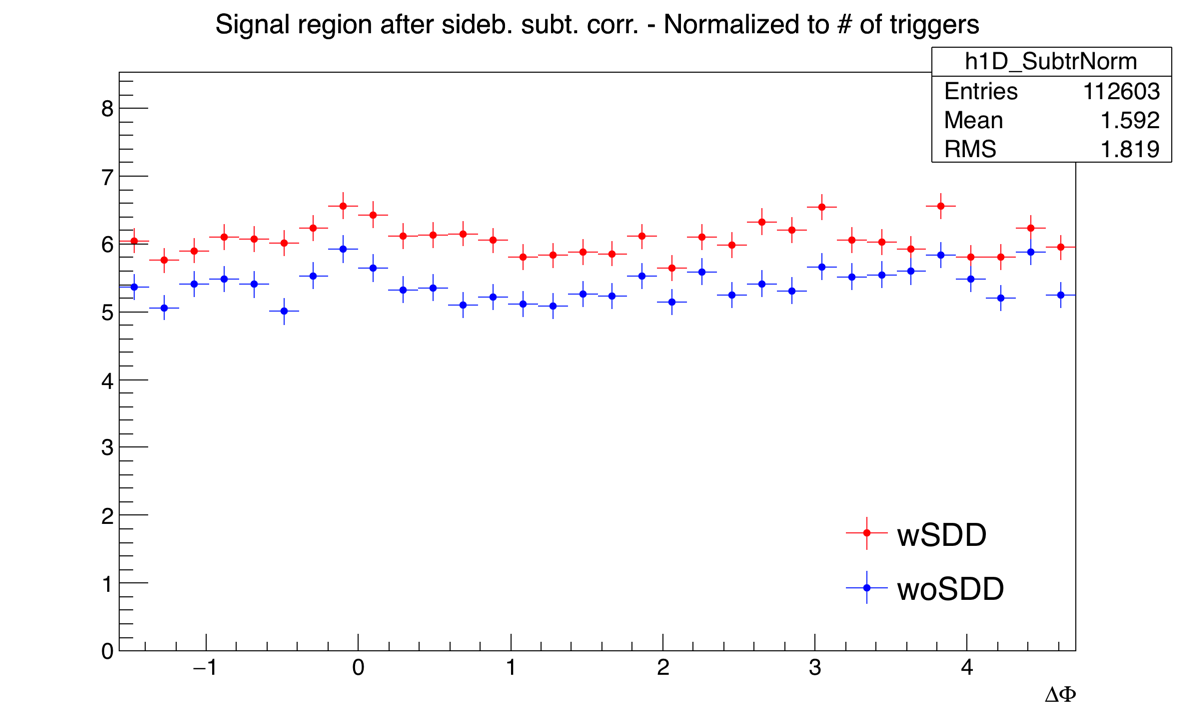
\includegraphics[width=0.8\linewidth, height=6cm]{figures/wSDD_vs_woSDD/AzimCorrDistr_Dstar_Canvas_PtIntBins2to3_PoolInt_thr0dot3to99dot0_Superimp.png}
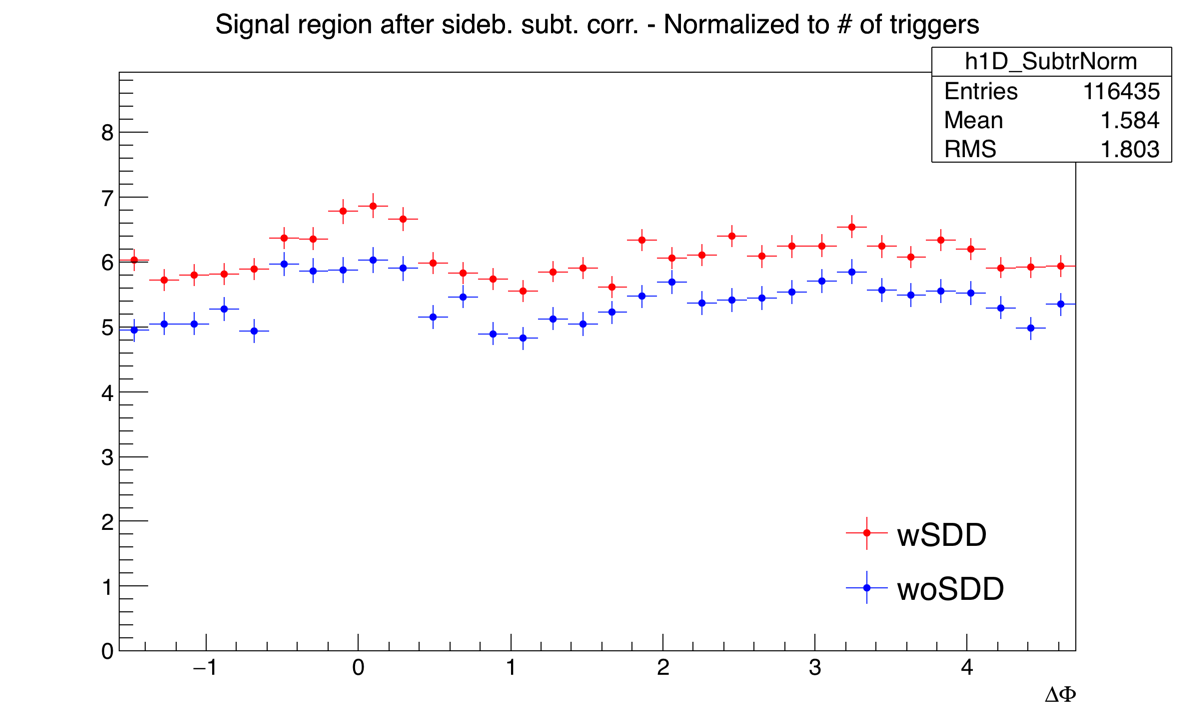
\includegraphics[width=0.8\linewidth, height=6cm]{figures/wSDD_vs_woSDD/AzimCorrDistr_Dstar_Canvas_PtIntBins4to6_PoolInt_thr0dot3to99dot0_Superimp.png}

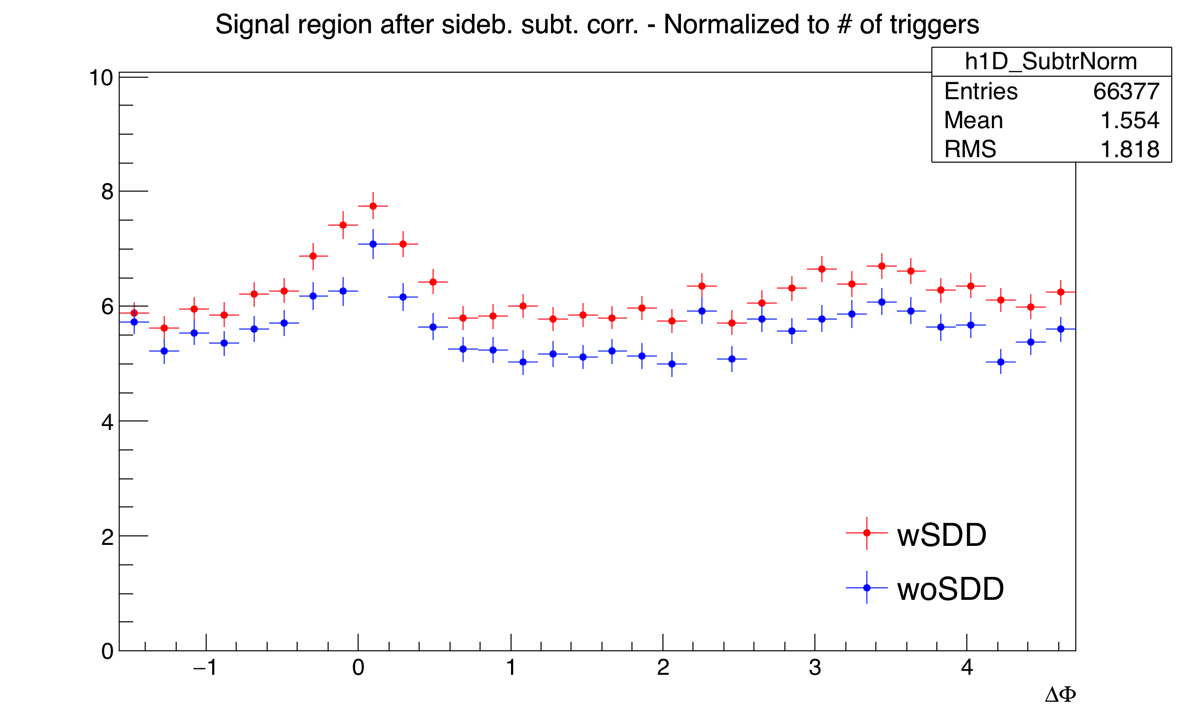
\includegraphics[width=0.8\linewidth, height=6cm]{figures/wSDD_vs_woSDD/AzimCorrDistr_Dstar_Canvas_PtIntBins7to9_PoolInt_thr0dot3to99dot0_Superimp.png}
\caption{Normalized azimuthal correlation distribution of $\Dstar$ for low $\pt$ ($3 < \pt(\Dstar) < 5$ GeV/c) on the top panel, mid $\pt$ ($5 < \pt(\Dstar) < 8$ GeV/c) on the middle panel and high $\pt$ ($8 < \pt(\Dstar) < 16$ GeV/c) on the bottom panel with a $\pt$ threshold for associated tracks of $\pt(assoc) > 0.3$ GeV/c. Blue points are referred to the woSDD sample while red points represent wSDD data.}
\label{wSSvswoSDD}
\end{figure}

\begin{figure}[!h]
\centering
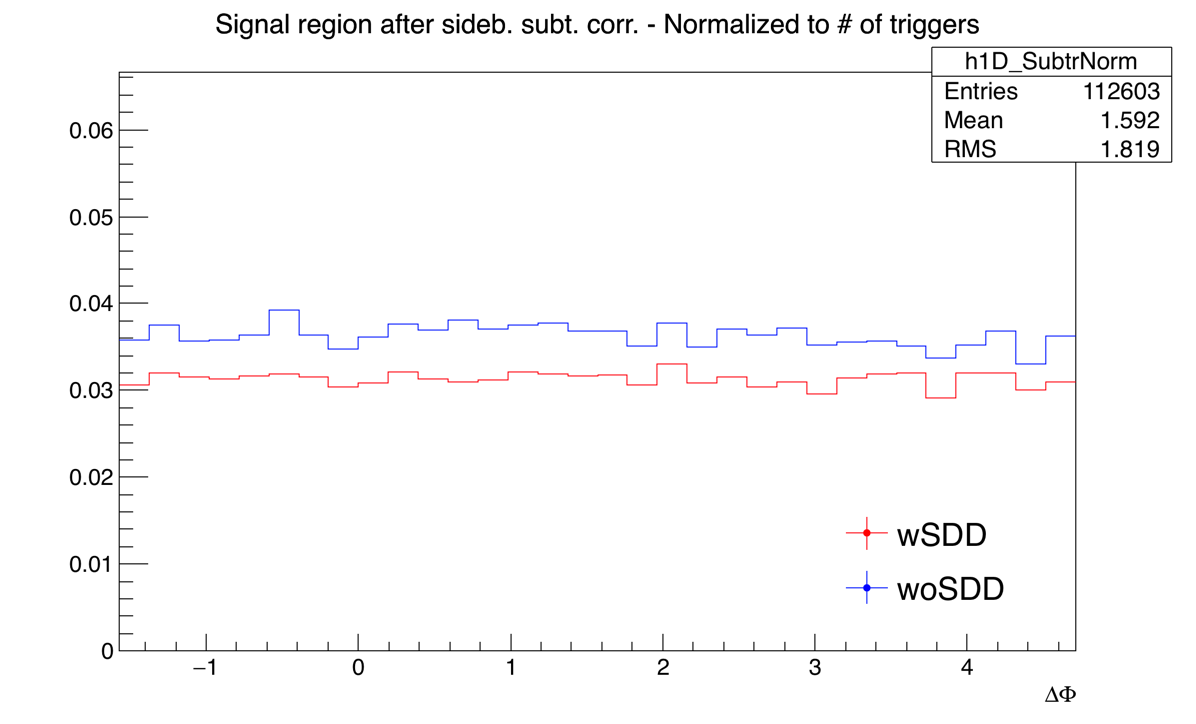
\includegraphics[width=0.8\linewidth, height=6cm]{figures/wSDD_vs_woSDD/Uncertanty_AzimCorrDistr_Dstar_Canvas_PtIntBins2to3_PoolInt_thr0dot3to99dot0.png}
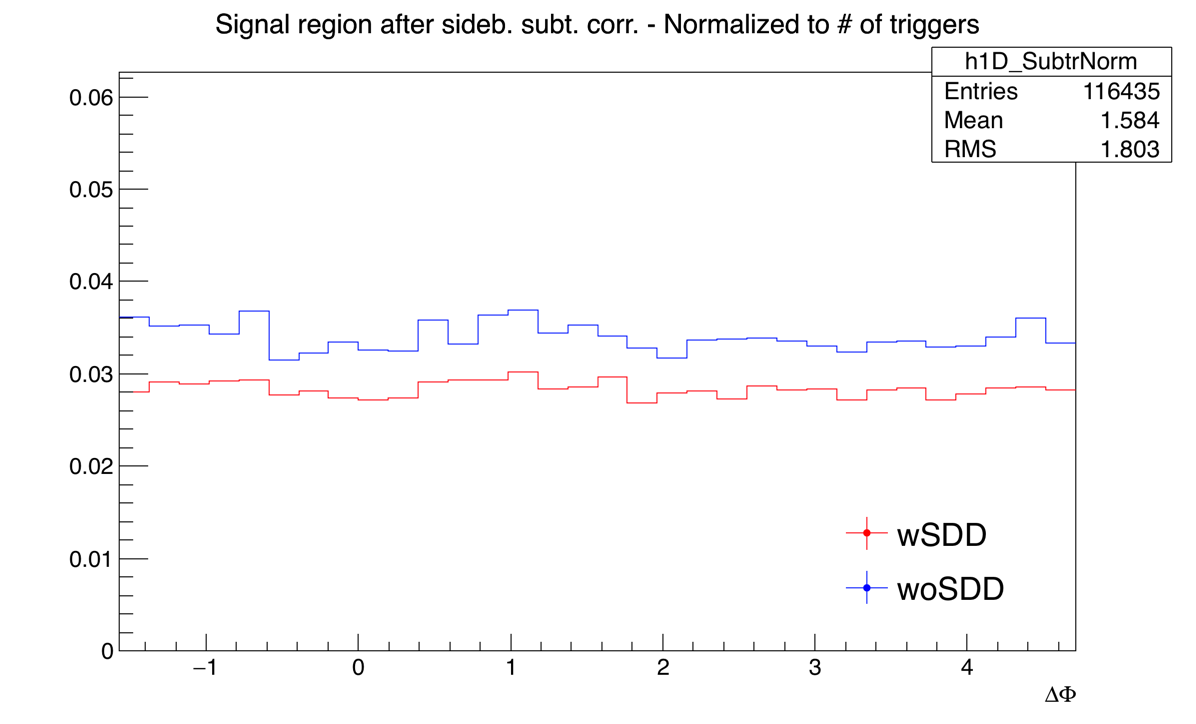
\includegraphics[width=0.8\linewidth, height=6cm]{figures/wSDD_vs_woSDD/Uncertanty_AzimCorrDistr_Dstar_Canvas_PtIntBins4to6_PoolInt_thr0dot3to99dot0.png}

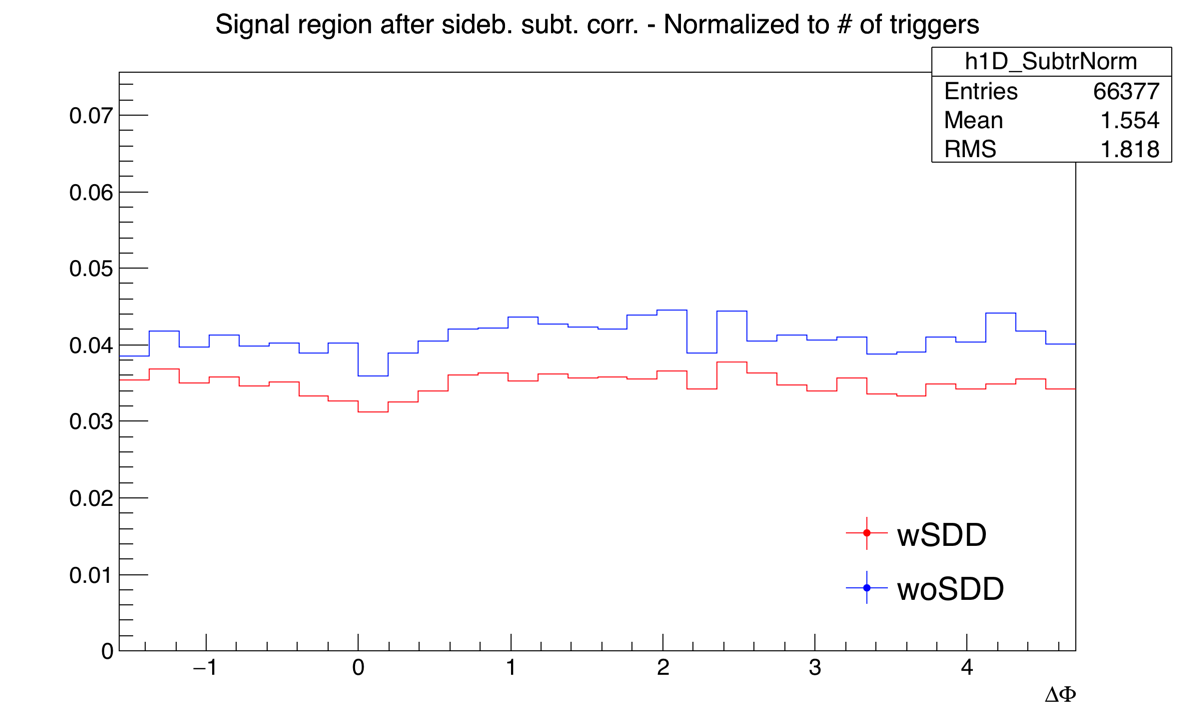
\includegraphics[width=0.8\linewidth, height=6cm]{figures/wSDD_vs_woSDD/Uncertanty_AzimCorrDistr_Dstar_Canvas_PtIntBins7to9_PoolInt_thr0dot3to99dot0.png}
\caption{Statistical uncertainty extracted from the azimuthal correlation distribution of $\Dstar$ with associated charged particles. Top panel: $3 < \pt(\Dstar) < 5$ GeV/c.
Mid panel: $5 < \pt(\Dstar) < 8$ GeV/c. Bottom panel: $8 < \pt(\Dstar) < 16$ GeV/c.
Blue line is referred to the woSDD sample while the red line represents wSDD data.}
\label{wSSvswoSDDuncertainty}
\end{figure}

It can be observed that the data sample that includes the SDD information is characterized by $\approx 10-15\%$ more statistics in each $\pt$ ranges analyzed. This difference is related to the larger efficiency in track reconstruction with the wSDD sample - a larger number of tracks survives to the selection request of 3 points in the ITS, which is part of the selection requests applied on the previous D-h analysis.

As a result, the wSDD sample is also affected by a slightly lower relative statistical uncertainty (about 12-15\%) due to several reasons: the larger tracking efficiency, the major number of signal entries in the invariant mass distributions and a slight increase of S/B, which reflects in a slight decrease of uncertainty from the sideband subtraction.
It has also to be considered that, on the full sample including also the FAST cluster, the increase in performance would be further reduced.
The overall statistical uncertainty difference resulting from the comparison is not enough to justify the implementation of two different analysis and two subsequent different corrections either for $\Dstar$ and $\Dplus$.

Anyway, to cope with the lower tracking efficiency w.r.t. 2013 data sample, after this study it was decided to reduce the ITS request for the associated tracks from 3 (used on 2013 data) to 2 ITS clusters as default selection criterion.


